\section{Results}
\label{sec:rslts}

%introduction
In this section the outcomes of the clustering (\ref{ssec:clures}), the Content-Based learning models (\ref{ssec:rcblm}), the ranking (\ref{ssec:rr}) and the practical solutions to improve results (\ref{ssec:ir}) are presented and elaborated.

%Clustering
\subsection{Clustering Results}
\label{ssec:clures}

First we look at our results to answer Research Question~\ref{rq:cold}:
\begin{itemize}
	\item[] \em Can clustering deal with label sparsity in job matching data?
\end{itemize}

\noindent In this part the results of the clustering of both the user and job features are described.
The first attempt is to cluster the user or job data using the K-prototypes algorithm which can deal with both numerical and categorical data.
To improve the clustering results the numerical data is converted to \textit{z}-scores.
When this algorithm is applied the clustering time after time breaks down around cluster size 50. If after this point the number of clusters is increased the algorithm fails to initiate the cluster centroids.
Various cluster initiation schemes and even manual initiation have been tried, but the problem persists.

Due to the fact that the K-prototypes could not be used for this research and because of the fact that only a few columns were numerical it was decided to treat all numerical data as categorical data and to apply the K-modes algorithm.
For the users the optimal cluster size seems to be around 150 and for jobs around 100 (figure \ref{fig:eb}).
However, the Elbow plots do not show a determinative point where they flatten out.
Thus to validate the clustering results the cluster sizes 25 till 300 with an interval of 25 were tested on 12 scenarios for both Logistic Regression and Neural Network.
In total 288 tests were conducted (12 different cluster size $\times$ 12 scenarios $\times$ 2 algorithms). 
The table of the best results can be found in appendix \ref{ssec:cluscen}.
The results do not show any improvement over the baseline, and therefore it can be concluded that in our case K-modes clustering of user or job features is not effective for the recommender system.

\begin{figure}[H]
    \centering
    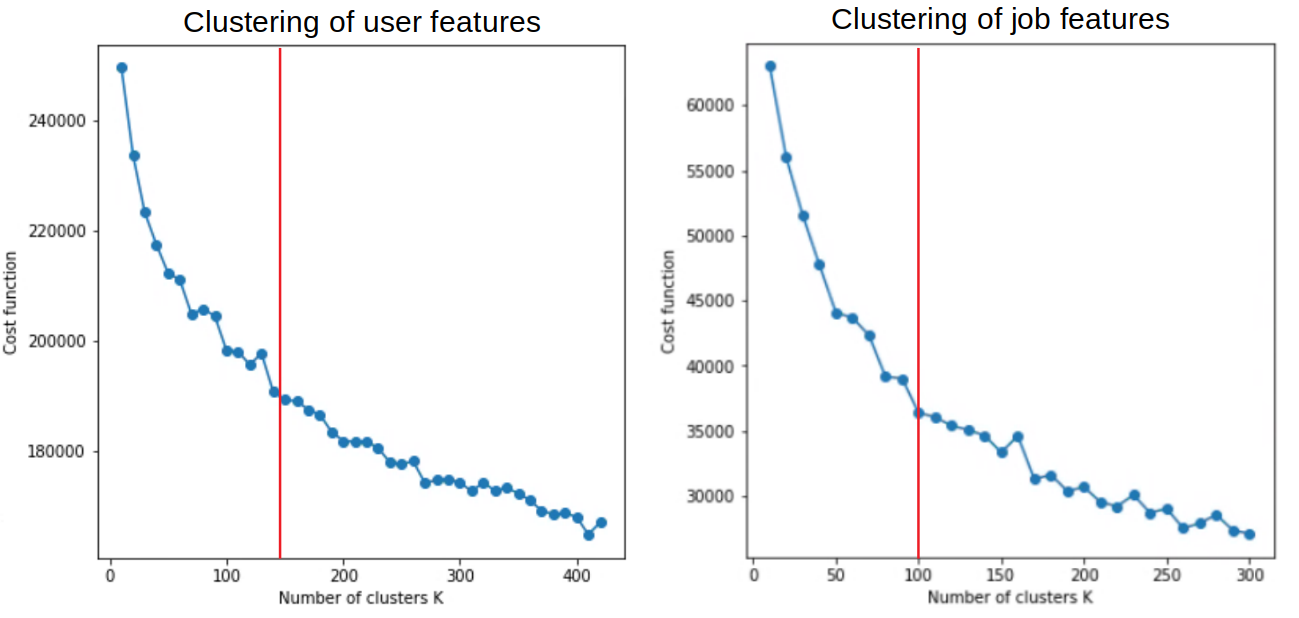
\includegraphics[width=\linewidth]{ThesisTemplate/Images/Clustering.png}
    \caption{\label{fig:eb} \footnotesize{Elbow Plots of the Clustering of Users and Jobs}}
\end{figure}

As second clustering method it is attempted to spread the Term Frequency-Inverse Document Frequency scores (TF-IDF) of the top 1000 words in the job descriptions over meaningful clusters.
Plotting the scores in an Elbow plot (appendix \ref{ssec:Kmeans}) does not show a point where the line flattens out.
Visual inspection comparing the clusters with the related job title displayed randomness.
The results could be explained by the fact that the top 1000 words of the job descriptions contain a great diversity of words, while the observations (8,265) are relatively low.
It is plausible that this technique can yield better results when the number of observations is higher.
Therefore, for this research it was decided to look at other approaches for clustering.

The third clustering approach is to cluster the n-grams of the job title characters.
Applying Hierarchical Clustering results in that the job titles are distributed over 286 clusters. 
Through a visual inspection comparing the assigned clusters with the associated job titles this clustering seems to deliver promising results, however when assessing the accuracy and MCC scores the performance is worse than the K-modes clustering.
The hierarchical clustering results can be found in appendix \ref{ssec:hieclu}.

% The job data contains a number of recurring job titles that are exactly the same, and based on the hierarchical clustering results it can be assumed that even though the job title is the same the underlying features deviate. 
% To verify this assumption the cosine similarities of a job vector versus all other job vectors for all observations were calculated.
% None of the returned similarities give an exact match, so highly similar job vectors can have very different associated job titles and visa versa.
% Therefore it can be reasoned that although job titles sometimes are the exact same or very similar the underlying features are different.
% \mynote[author=Harrie]{Laten we even naar deze redenering kijken.}

In conclusion to answer Research Question~\ref{rq:cold}: it was found that in our case the tested clustering approaches are not effective in dealing with label sparsity.

%Results Content-Based Learning Models
\subsection{Results Content-Based Learning Models}
\label{ssec:rcblm}

In this part we look at our results to answer Research Question~\ref{rq:model}:
\begin{itemize}
	\item[] \em Are there significant differences between models in predictive performance?
\end{itemize}

\noindent When assessing the accuracy results it must be taken into account that the dataset exhibits a class imbalance of 79\% being positive labels and 21\% being negative labels.
The consequence of this imbalance is that if the classifier predicts all labels to be positive it achieves 0.79 accuracy.
% This fallaciously suggests that the classification results are decent.
% \mynote[author=Harrie]{Dit is raar, je hebt de resultaten nog niet geintroduceerd, maar zegt toch dat ze onterecht decent lijken.}
Here is where the utility of the Matthews Correlation Coefficient (MCC) comes into play, as the MCC in such case will be 0.00 because no labels are classified as negative.

The classification results of the models are shown in table \ref{tab:res}.
Judging only on the accuracy alone it does not seem to make a great difference which model is applied.
When the MCC scores are analyzed the Neural Network performs 10\% better than its closest rival and 52\% better than the Nearest Neighbors baseline.
The higher performance of MCC suggests better balanced predictions of both the positive and negative labels.
The best scores for the Neural Network were achieved with a setup of one hidden layer.
When more hidden layers are added the performance decays gradually.
In general a Neural Network can learn more complex patterns when the number of hidden layers increase, however this also raises the risk of overfitting of the model on the train data.
% \mynote[author=Harrie]{Deze zin loopt niet lekker.}
Therefore, it is a likely explanation that when extra layers are added the performance is worsened due to overfitting.

\begin{table}[h]
\begin{footnotesize}
\begin{tabular}{lrr}
\toprule
\textbf{Model}      & \textbf{Accuracy} & \textbf{MCC}  \\
\midrule
Nearest Neighbors (baseline)   & 0.76              & 0.29          \\     
K-Nearest Neighbors & 0.80              & 0.35          \\
RandomForest        & 0.82              & 0.40          \\
Logistic Regression & 0.80              & 0.35          \\
Linear SVC          & 0.80              & 0.33          \\
Neural Network      & 0.81              & 0.44          \\
\bottomrule
\end{tabular}

\end{footnotesize}
\caption{\label{tab:res} \footnotesize{Classification Scores of Trained Models}}
\end{table}

For the Neural Network the MCC score is low and therefore also the confusion matrix (table \ref{tab:cmnn}) is analyzed.
Overall it can be seen that the model is good in classifying the positive labels and less well when it comes to classifying the negative labels.
Less than half (49\%) of the true negative labels are classified correctly, while 91\% of true positive labels are correct.
Based on the metrics it is plausible that due to the class imbalance the Neural Network displays a tendency to classify all observations as positive labels, and therefore it is hard to determine how well the positive labels are learned.
This behavior is even more evident with the other classification models.

\begin{table}[h]
\begin{footnotesize}
\begin{tabular}{l|l|l|r|r|}
    \multicolumn{3}{c}{\multirow{2}{*}}                          &  \multicolumn{2}{c}{\textbf{Actual labels}}   \\ 
    \cline{4-5}
    \multicolumn{3}{c|}{}                                        &Positive           &Negative                   \\
    \cline{3-5}
    \multicolumn{2}{l|}{\textbf{Predicted}}  &Positive           & 1,129      &111                  \\
    \cline{3-5}
    \multicolumn{2}{l|}{\textbf{labels}}     &Negative           & 190         &181                 \\
    \cline{3-5}
\end{tabular}





\end{footnotesize}
\caption{\label{tab:cmnn} \footnotesize{Classification Results of the Neural Network}}
\end{table}

In conclusion to answer Research Question~\ref{rq:model}: it was found that there are significant differences between the models and that in our case the Neural Network has the best performance.

%Ranking Results
\subsection{Ranking Results}
\label{ssec:rr}

In this section the results are assessed to answer Research Question~\ref{rq:ranking}:
\begin{itemize}
	\item[] \em Does a model trained for predicting of job matches translate to a good ranking-based recommender?
\end{itemize}

\noindent Another method to evaluate the classification of the positive labels is by ranking them and then retrieving the average rank.
To achieve that a trained model predicts the label probability of each user-job combination, whereafter the average rank can be calculated.
There are 4,983 unique jobs (midpoint is 2,491), and the expectation would be that the positive labels would at least come in the top 100. 
The results show a different picture, for Logistic Regression the average rank of the positive labels is 2,611 and for the Neural Network 2,250.
The Neural Network performs best, but the results are not considerably better than the random selection and definitely not close to an average rank below 100.
% \mynote[author=Harrie]{Heb je significant testing gedaan? gebruik anders een ander woord: bijv. considerably}

The outcomes of the rankings do not appear to be better than the random baseline. 
% \mynote[author=Harrie]{Je bedoelt de resultaten zien er niet veel beter uit dan de random baseline, dat is niet hetzelde als er willekeurig uitzien.}
% To validate the ranking implementation a subset of 10 users and 100 jobs are picked from the dataset and the model is purposefully overfitted using the whole subset to train and validate.
% This procedure returns an average rank of one, what is expected when a proper implementation is overfitted.
% \mynote[author=Harrie]{Het overfitting verhaal zou ik weglaten.}
Random results of Logistic Regression occur because the model returns precisely the same rankings for every user.
This is caused by the linearity of the model, for each row in the matrix the user features are the same while the jobs features are different for each entry.
A linear model only learns the dissimilarities, hence only the job features since all user features are the same for each row entry. 
Because the user features are effectively not taken into account and each user is compared with the same jobs the model predicts the same ranks for each row.
Therefore, it can argued that Logistic Regression with a linear model is not suitable for ranking.
% \mynote[author=Harrie]{Logistic Regression met een linear model, je NN doet ook LR namelijk.}
The Neural Network is not affected by this thanks to its ability to learn non-linear relations in the data. 
% \mynote[author=Harrie]{zeg maar not affected}

In conclusion to answer Research Question~\ref{rq:ranking}: it was found that in our case the trained models did not translate to a good ranking-based recommender.

%Improving the Results
\subsection{Results of the Approaches to Improve the Performance}
\label{ssec:ir}

Finally in this part we look at our results to answer Research Question~\ref{rq:strategies}:
\begin{itemize}
	\item[] \em Does feature selection and addressing class imbalance have a significant effect on the predictive performance?
\end{itemize}

\noindent In this part the results of two practical ways to improve the classification results are presented. 
First the results of addressing class imbalance are described, and thereafter the importance of the features is analyzed. 
Because the outcomes for all models show the same trends only the results of the Neural Network are presented.

Two methods to rebalance classes were tested. 
As shown before in section~\ref{sec:setup} Experimental Setup the train set is composed of 6,654 observations of which 5,250 have a positive label and 1,404 a negative label (table \ref{tab:tvs}).
By randomly deleting the observations of the overrepresented class the number of positive labels in the train set is reduced to 1,404.
The results of undersampling and oversampling for the Neural Network are shown in table \ref{tab:nnci}, for a full listing of the results for all models is referred to appendix \ref{ssec:ruo}.
The results of undersampling for the Neural Network do not display a performance improvement.
These  results can be attributed to the fact that an already small train set is reduced with 58\% in size by the undersampling.
With fewer training examples it becomes more difficult for Neural Network to learn generalizing patterns in the data.

\begin{table}[h]
\begin{footnotesize}
\begin{tabular}{lll}
\toprule
     & \textbf{Accuracy} & \textbf{MCC}  \\
\midrule
\textit{Baseline}           & \textit{0.81}     & \textit{0.44} \\
Undersampling               & 0.73              & 0.40          \\
Oversampling                & 0.80              & 0.39          \\
\bottomrule
\end{tabular}

\end{footnotesize}
\caption{\footnotesize{\label{tab:nnci} Class Rebalancing for the Neural Network}}
\end{table}

The oversampling of observations is realized by applying Synthetic Minority Over-sampling Technique (SMOTE). 
By applying SMOTE the number of observations of the negative labels in the train set is increased to 5,250. 
This artificial creation of extra observations does not lead to better results for the Neural Network.
It can therefore be argued that the way in which SMOTE generates new observations is unsuitable for the available data.

\begin{table}[h]
\begin{footnotesize}
\begin{tabular}{llll}
\toprule
        & \textbf{\# Features}   & \textbf{Accuracy} & \textbf{MCC}  \\
\midrule
\textit{Baseline}               & \textit{438}           & \textit{0.81}     & \textit{0.44} \\
Chi-Square Test                 & 180                    & 0.80              & 0.38          \\
BFE   & 116                    &  0.81            & 0.43          \\
RFECV & 115              & 0.83    & 0.46          \\
\bottomrule
\end{tabular}

\end{footnotesize}
\caption{\label{tab:nnfi} \footnotesize{Feature Importance Analysis Results for the Neural Network}}
\end{table}

For the analysis of the importance of the features three methods are tested. 
The results for the Neural Network are shown in table \ref{tab:nnfi}, the outcomes for all models can be found in appendix \ref{ssec:fi}.
From the results it can be deduced that there is a lot of noise present in the data, all approaches discard more than half of the features without significantly degrading the outcomes.
When assessing which features are dropped it can be established that this are predominantly user features.
Analyzing the user features that the RFECV method has retained it was found that based on heuristics 64\% of them can be classified as traits that hinder a person from getting a job.
This insight led to the question what would happen to the performance if all user features are eliminated.
Two interesting things can be observed in the outcomes of this question which is shown in table \ref{tab:nnfeat}.
First, when only using the users features the performance is suboptimal, and when only the jobs features are used the performance increases significantly.
Secondly, dropping all user features outperforms all tested feature importance analysis methods.
These outcomes suggests that the user features are not informative and carry no predictive power.
This is unexpected because it is assumed that the user characteristics for an important part determine the matchability with a job opening.

\begin{table}[h]
\begin{footnotesize}
\begin{tabular}{lrr}
\toprule
\textbf{Features}      & \textbf{Accuracy} & \textbf{MCC}  \\
\midrule
\textit{users + jobs (baseline)}& \textit{0.81}   & \textit{0.44}    \\
users   & 0.71  & 0.03 \\
jobs    & 0.84  & 0.53 \\ 
\bottomrule
\end{tabular}

\end{footnotesize}
\caption{\label{tab:nnfeat} \footnotesize{Neural Network: Scores per Feature Class}}
\end{table}

In conclusion to answer Research Question~\ref{rq:strategies} the findings are that in our case the tested methods for tackling class imbalance have a negative impact on performance.
However, eliminating user features has a positive effect on performance.

